\begin{table*}[t]
\caption{E3, frequency-error law only. Population: the 18{,}402 configurations
unsolved at every rung, so the same cases appear at each $T$ (an
adaptive-campaign cohort, not the fixed-$T$ design; the pair-gap and
detectability laws still need the fixed-$T$ sweep).}
\label{tab:e3}
\centering\small
\begin{tabular}{lccl}
\toprule
law & derived & fitted (bootstrap 95\,\%) & note\\
\midrule
$\sigma(\hat N)\propto T^{\gamma}$ & $-3/2$ & $-1.58$ [$-1.59$, $-1.56$] &
$T{=}20$--$80$ only: $-1.42$\\
pair-gap inflation & $-2$ & pending & needs fixed-$T$ cohorts\\
detectability & $-1/2$ & pending & needs fixed-$T$ cohorts\\
\bottomrule
\end{tabular}
\end{table*}
\begin{figure}[t]
\centering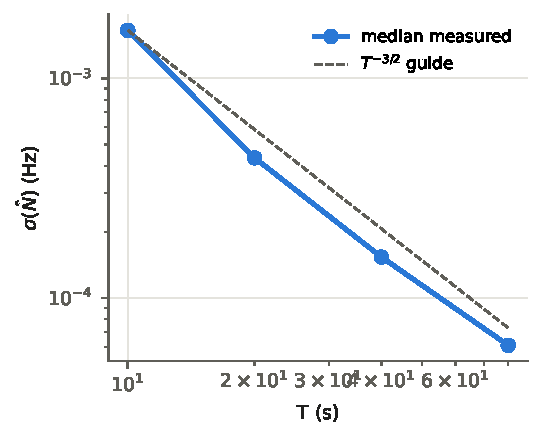
\includegraphics[width=0.75\columnwidth]{figures/E3_sigmaN.pdf}
\caption{Median certified $\sigma(\hat N)$ against $T$ for the always-unsolved
cohort, with the derived $T^{-3/2}$ guide.}
\label{fig:e3}
\end{figure}
